% Source : http://forum.mathematex.net/latex-f6/tableaux-de-proportionnalite-t3752.html?hilit=tableau

\documentclass[]{article}
	\usepackage{tikz,fullpage}
	\usetikzlibrary{arrows}


\begin{document}

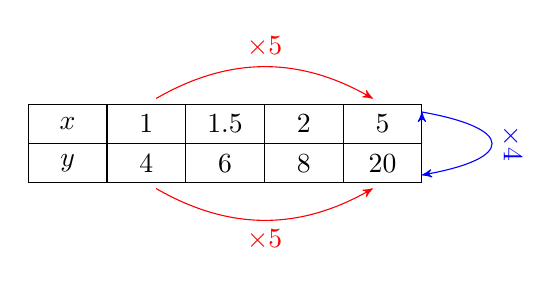
\begin{tikzpicture}
	\foreach \x/\xtext/\ytext in{0/x/y,1/1/4,2/1.5/6,3/2/8,4/5/20} {%
		\draw (\x,0.5) +(-0.5,-0.25) rectangle ++(0.5,0.25) ;
		\draw (\x,0) +(-0.5,-0.25) rectangle ++(0.5,0.25);
		\node[]  at (\x,0.5) {$\xtext$};
		\node[]  at (\x,0)   {$\ytext$};
		\node[] (x_\x)  at (\x,0.75) {};
		\node[] (y_\x) at (\x,-0.25) {};%
	}
	\draw[->,red,thin,>=stealth'] (x_1) edge [bend left] node[above]{$\times 5$} (x_4);
	\draw[->,red,thin,>=stealth'] (y_1) edge [bend right] node[below]{$\times 5$} (y_4);
	\draw[color=blue,->,thin,>=stealth'] (4.5,.65) edge [distance=1.2cm,bend left=80 ] node [above,sloped,midway]{$\times 4$} (4.5,-.15);
\end{tikzpicture}

\end{document}
